\documentclass[a4paper]{article}

\usepackage[english]{babel}
\usepackage[utf8]{inputenc}
\usepackage{amsmath}
\usepackage{graphicx}
\usepackage[colorinlistoftodos]{todonotes}
\usepackage{float}

\title{HW11: Variational Autoencoders}

\author{Yu Che Wang / yuchecw2}

\date{\today}

\begin{document}
\maketitle

\begin{abstract}
Apply variational autoencoders to MNIST dataset using TensorFlow framework.
\end{abstract}

\section{Single MNIST digits}
For 10 pairs of MNIST test images of the same digit, selected at random, compute the code for each image of the pair. Now compute 7 evenly spaced linear interpolates between these codes, and decode the result into images.

\begin{figure}[H]
\centering
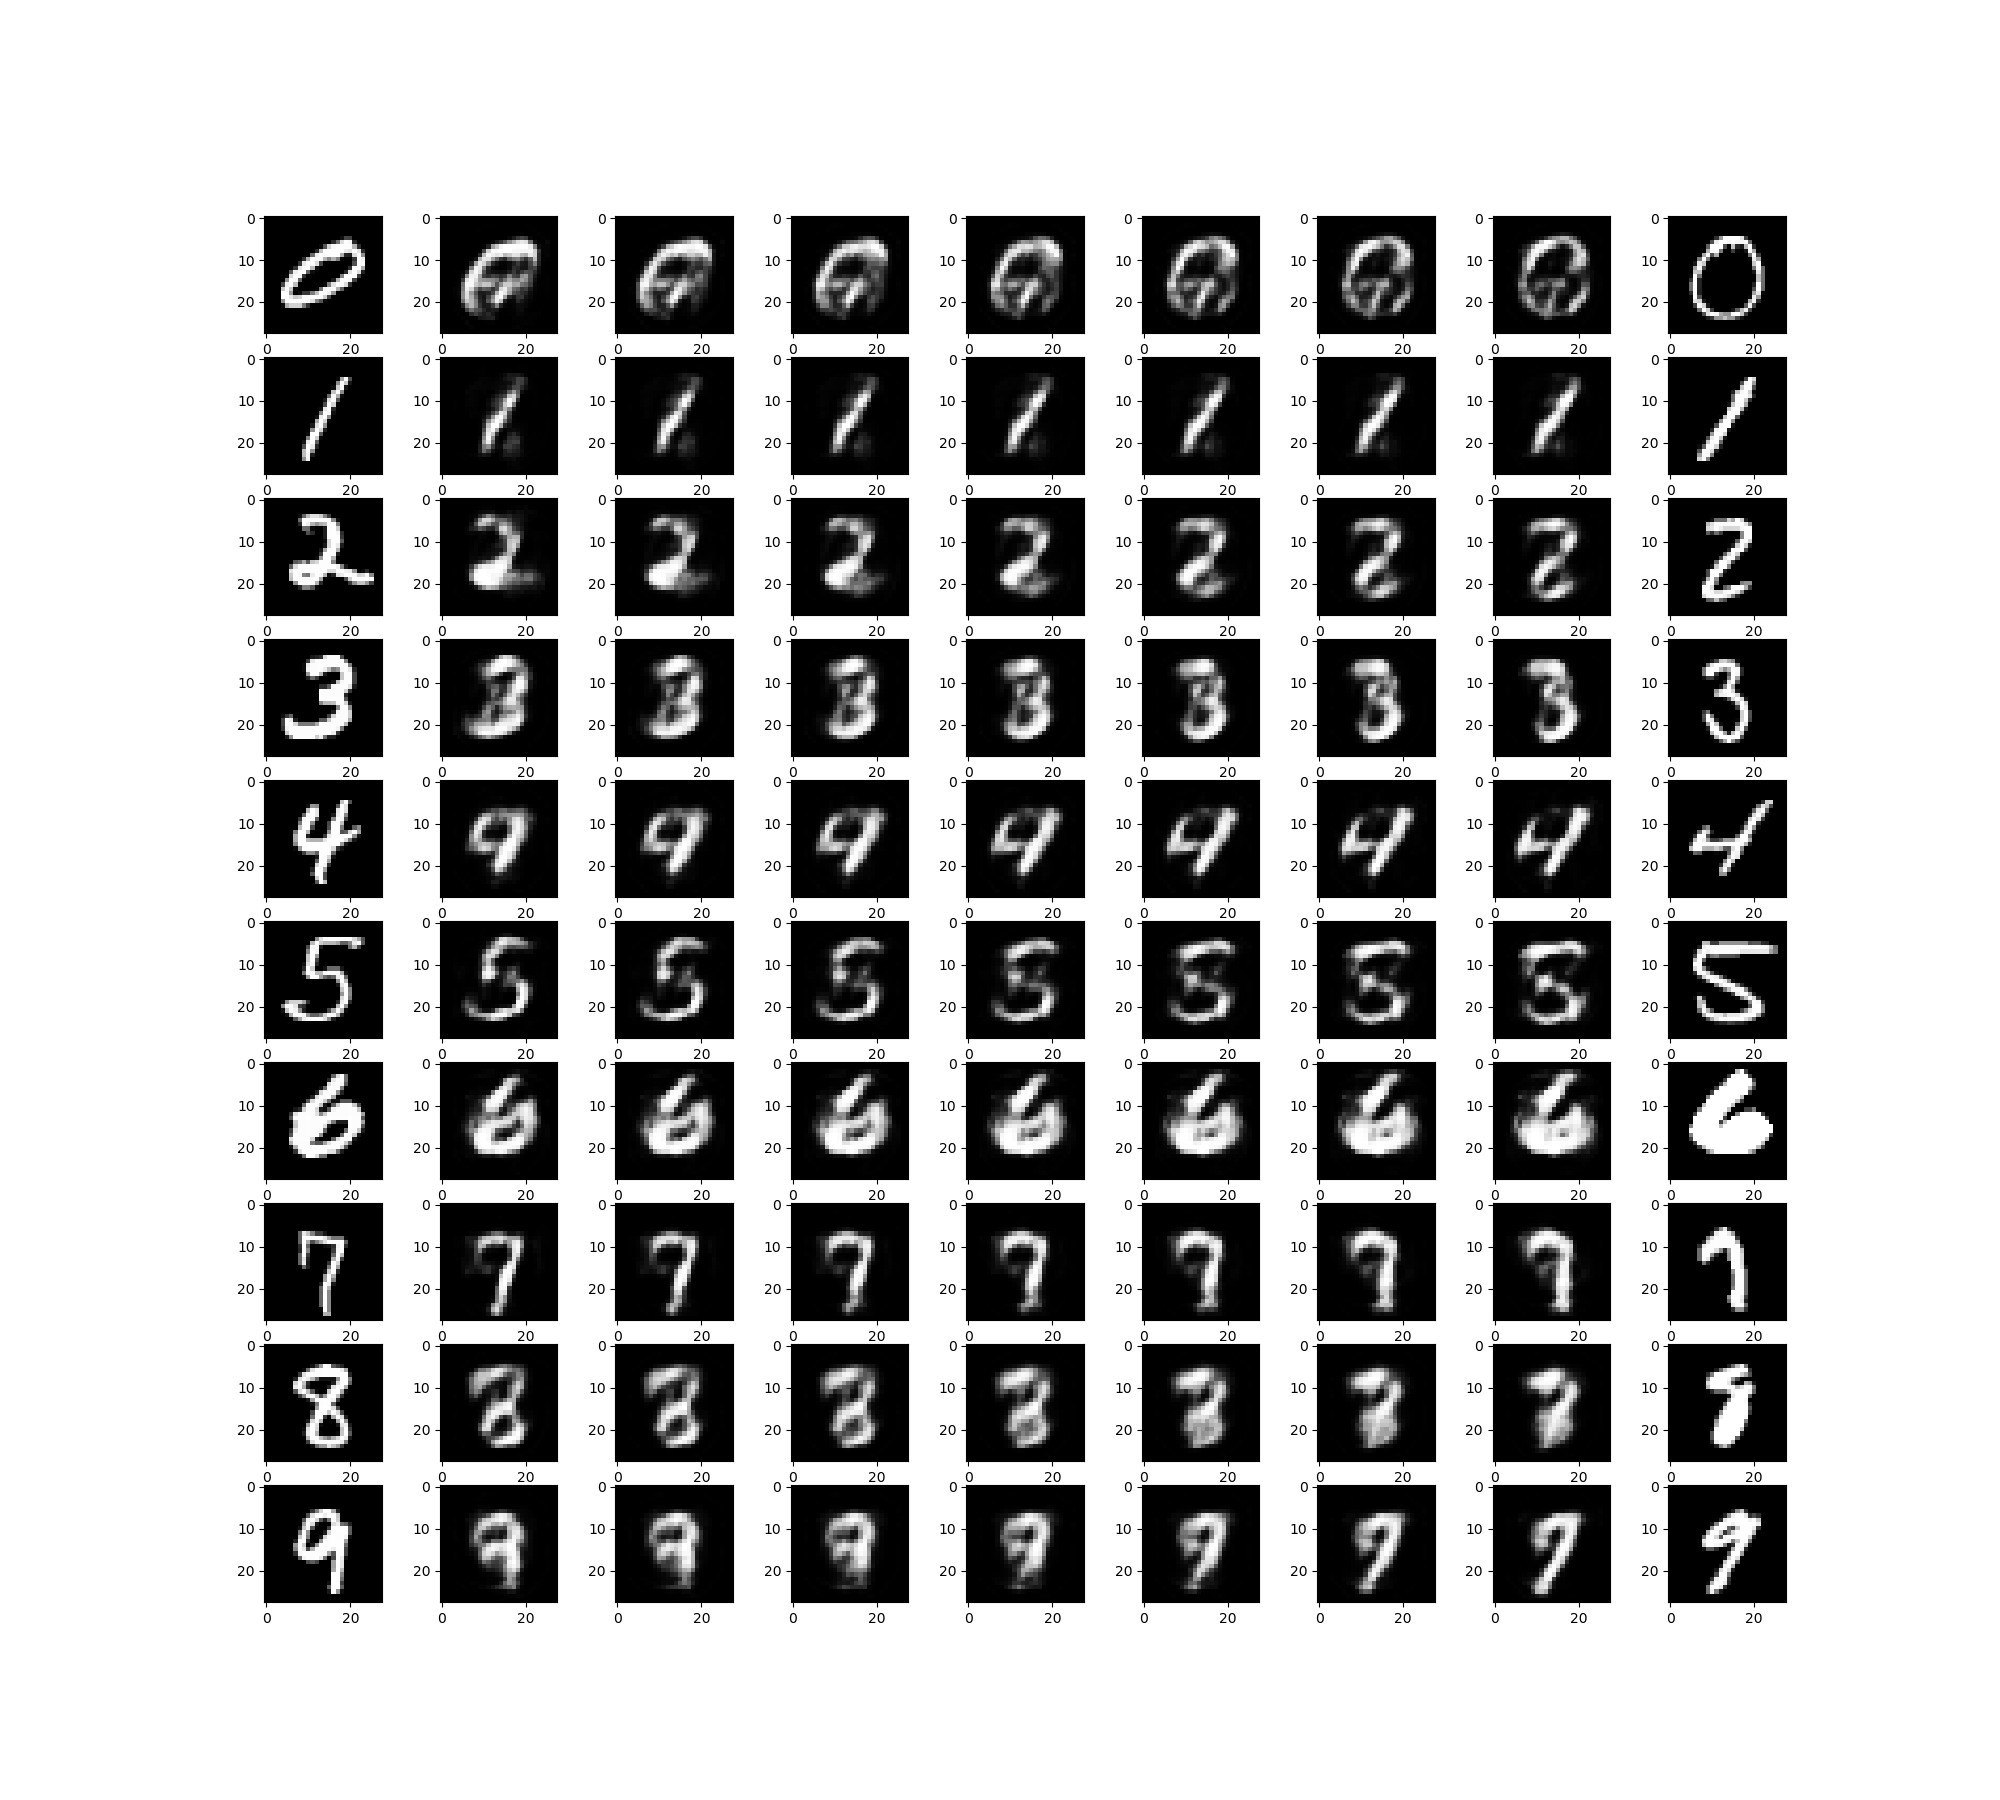
\includegraphics[width=1\textwidth]{same.png}
\caption{\label{fig:data}Single MNIST digits.}
\end{figure}

\section{Different MNIST digits}
For 10 pairs of MNIST test images of different digits, selected at random, compute the code for each image of the pair. Now compute 7 evenly spaced linear interpolates between these codes, and decode the result into images. 
\begin{figure}[H]
\centering
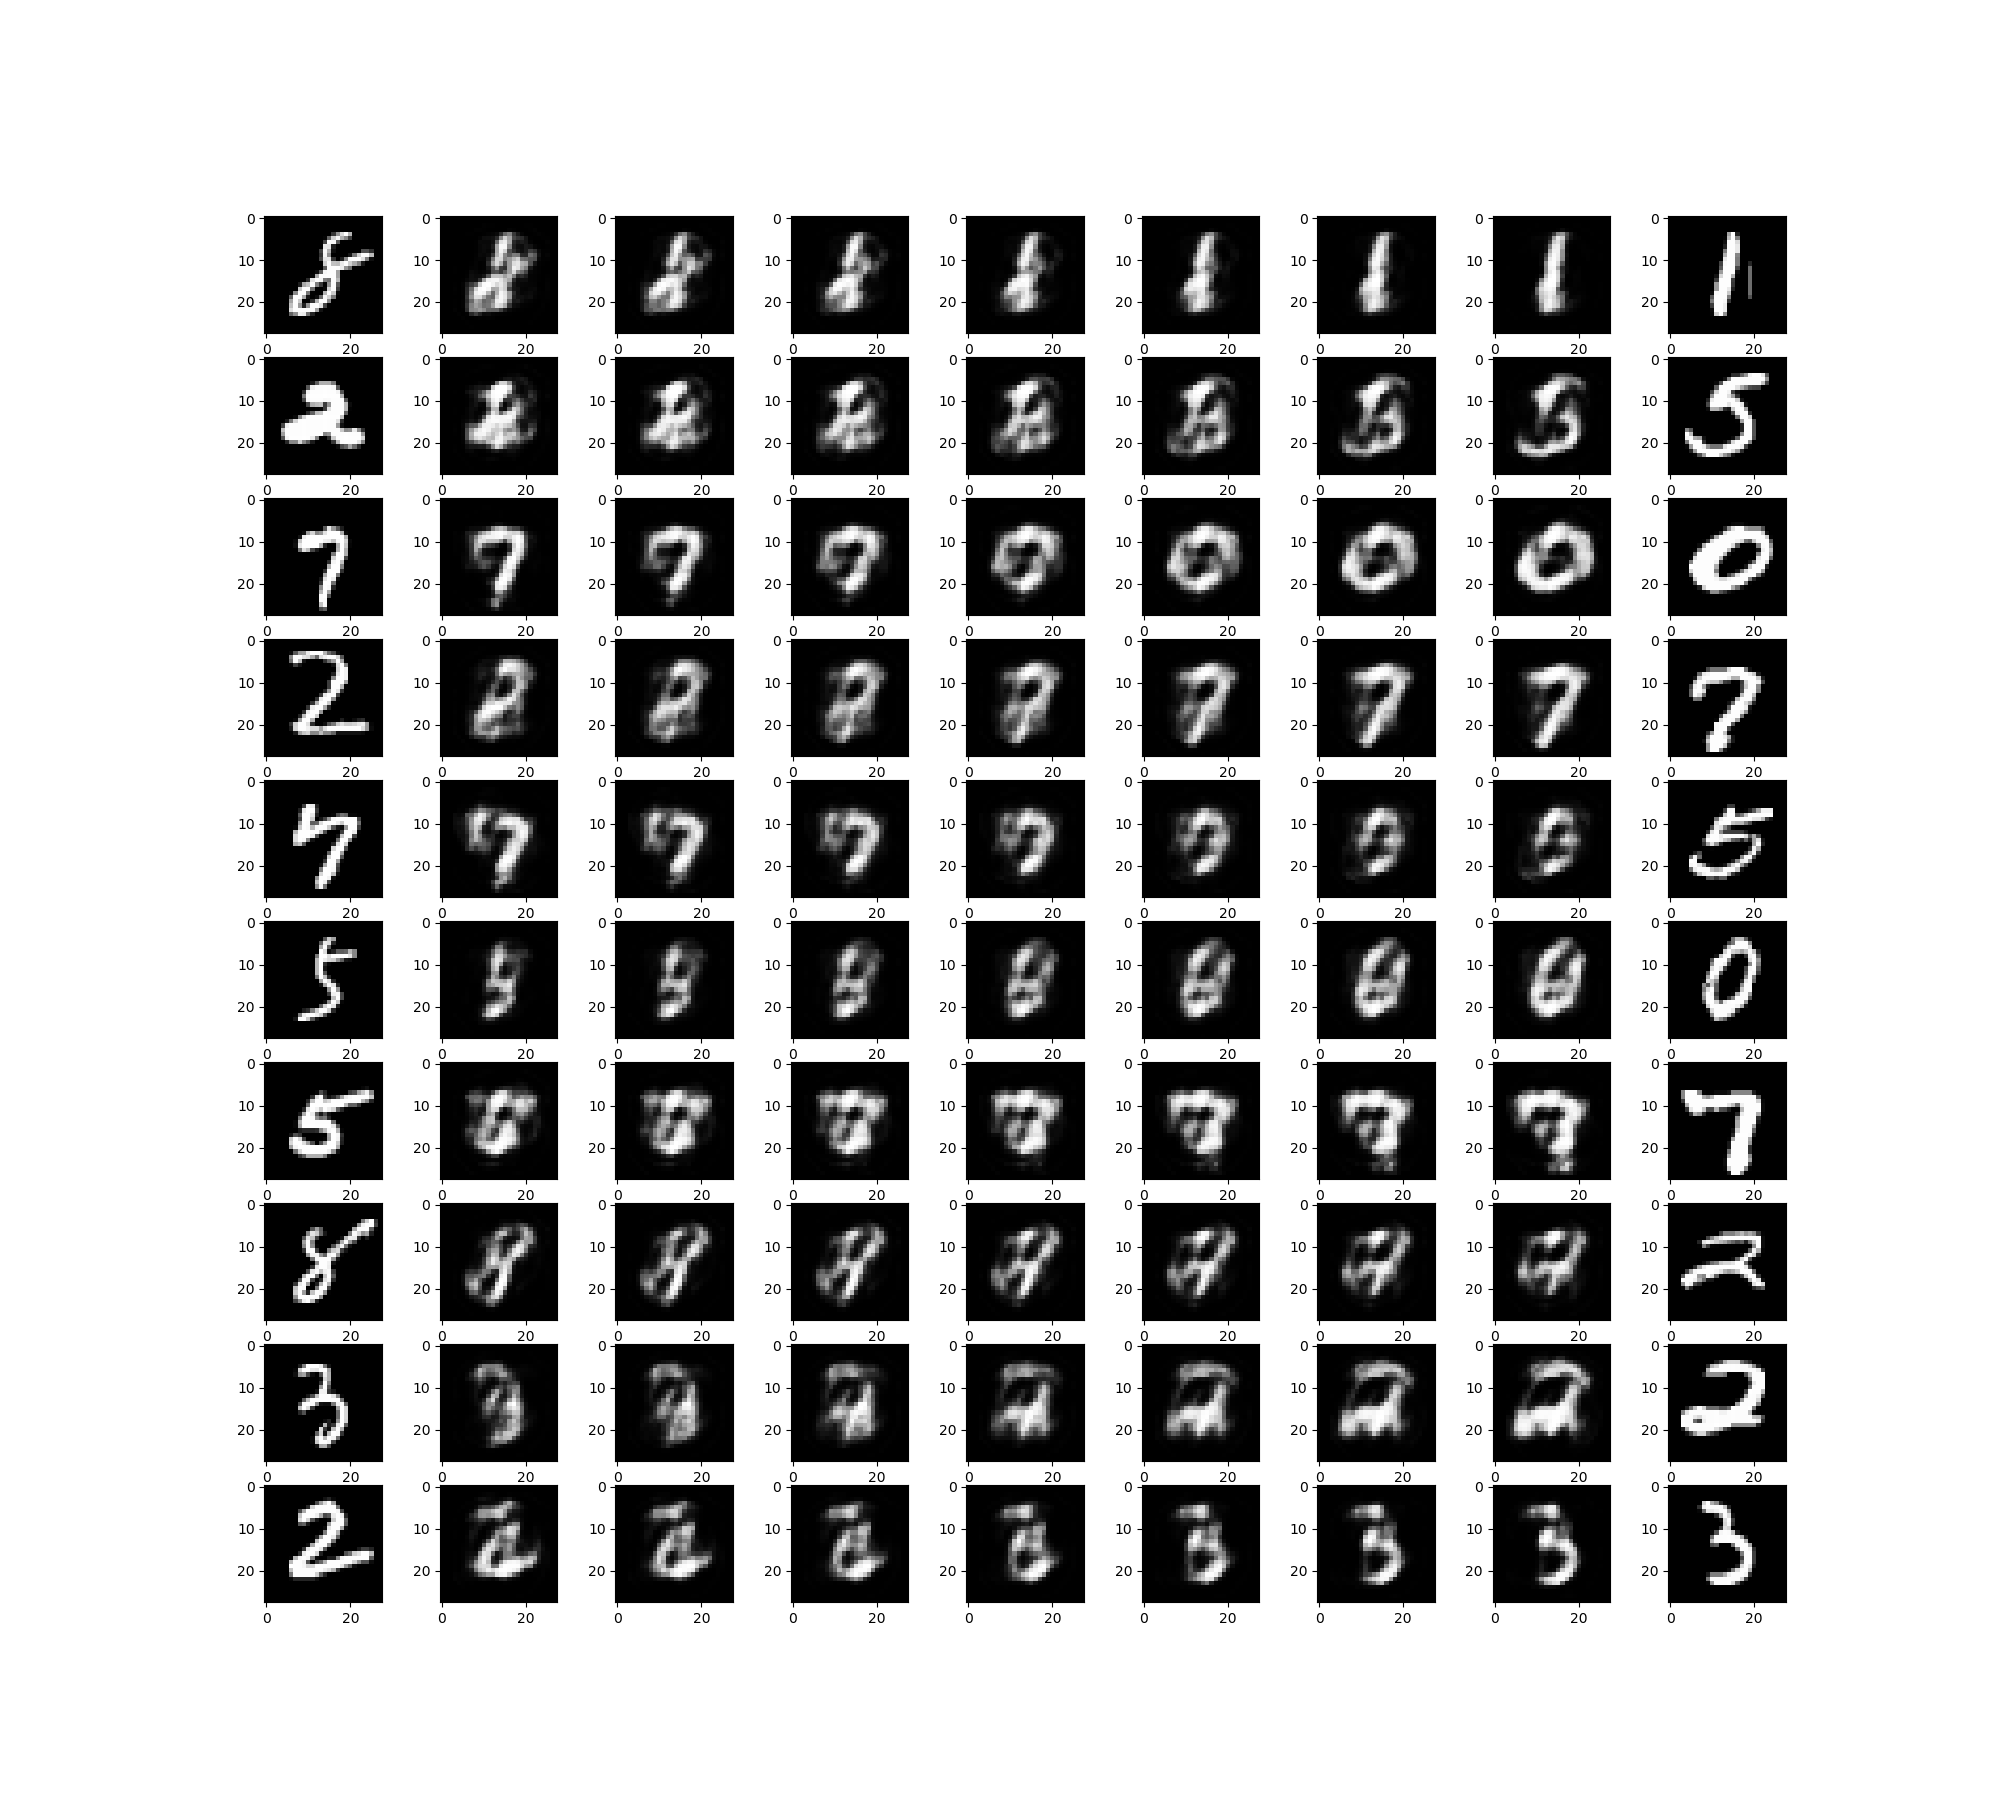
\includegraphics[width=1\textwidth]{different.png}
\caption{\label{fig:data}Different MNIST digits.}
\end{figure}

\section{Codes}
\begin{figure}[H]
\centering
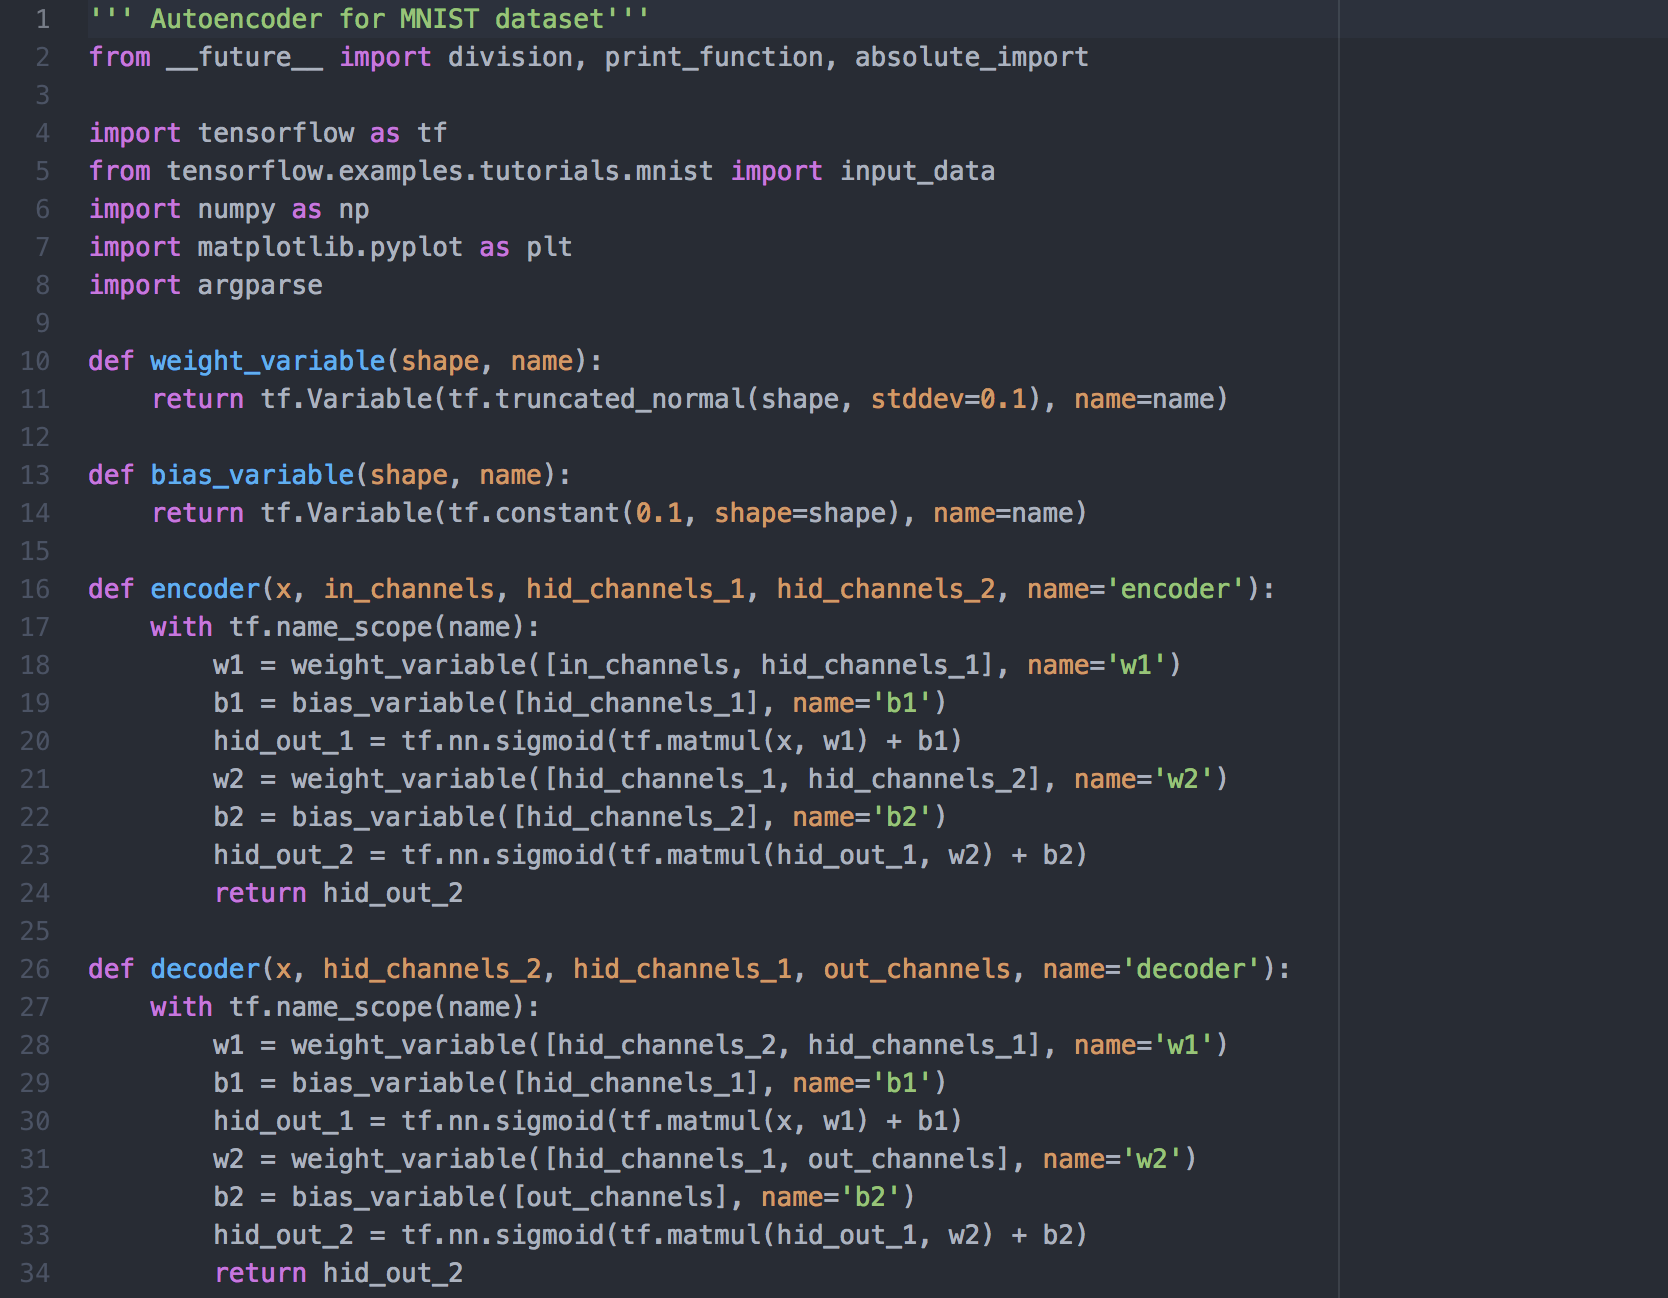
\includegraphics[width=0.9\textwidth]{1.png}
\caption{\label{fig:data}Helper functions.}
\end{figure}
\begin{figure}[H]
\centering
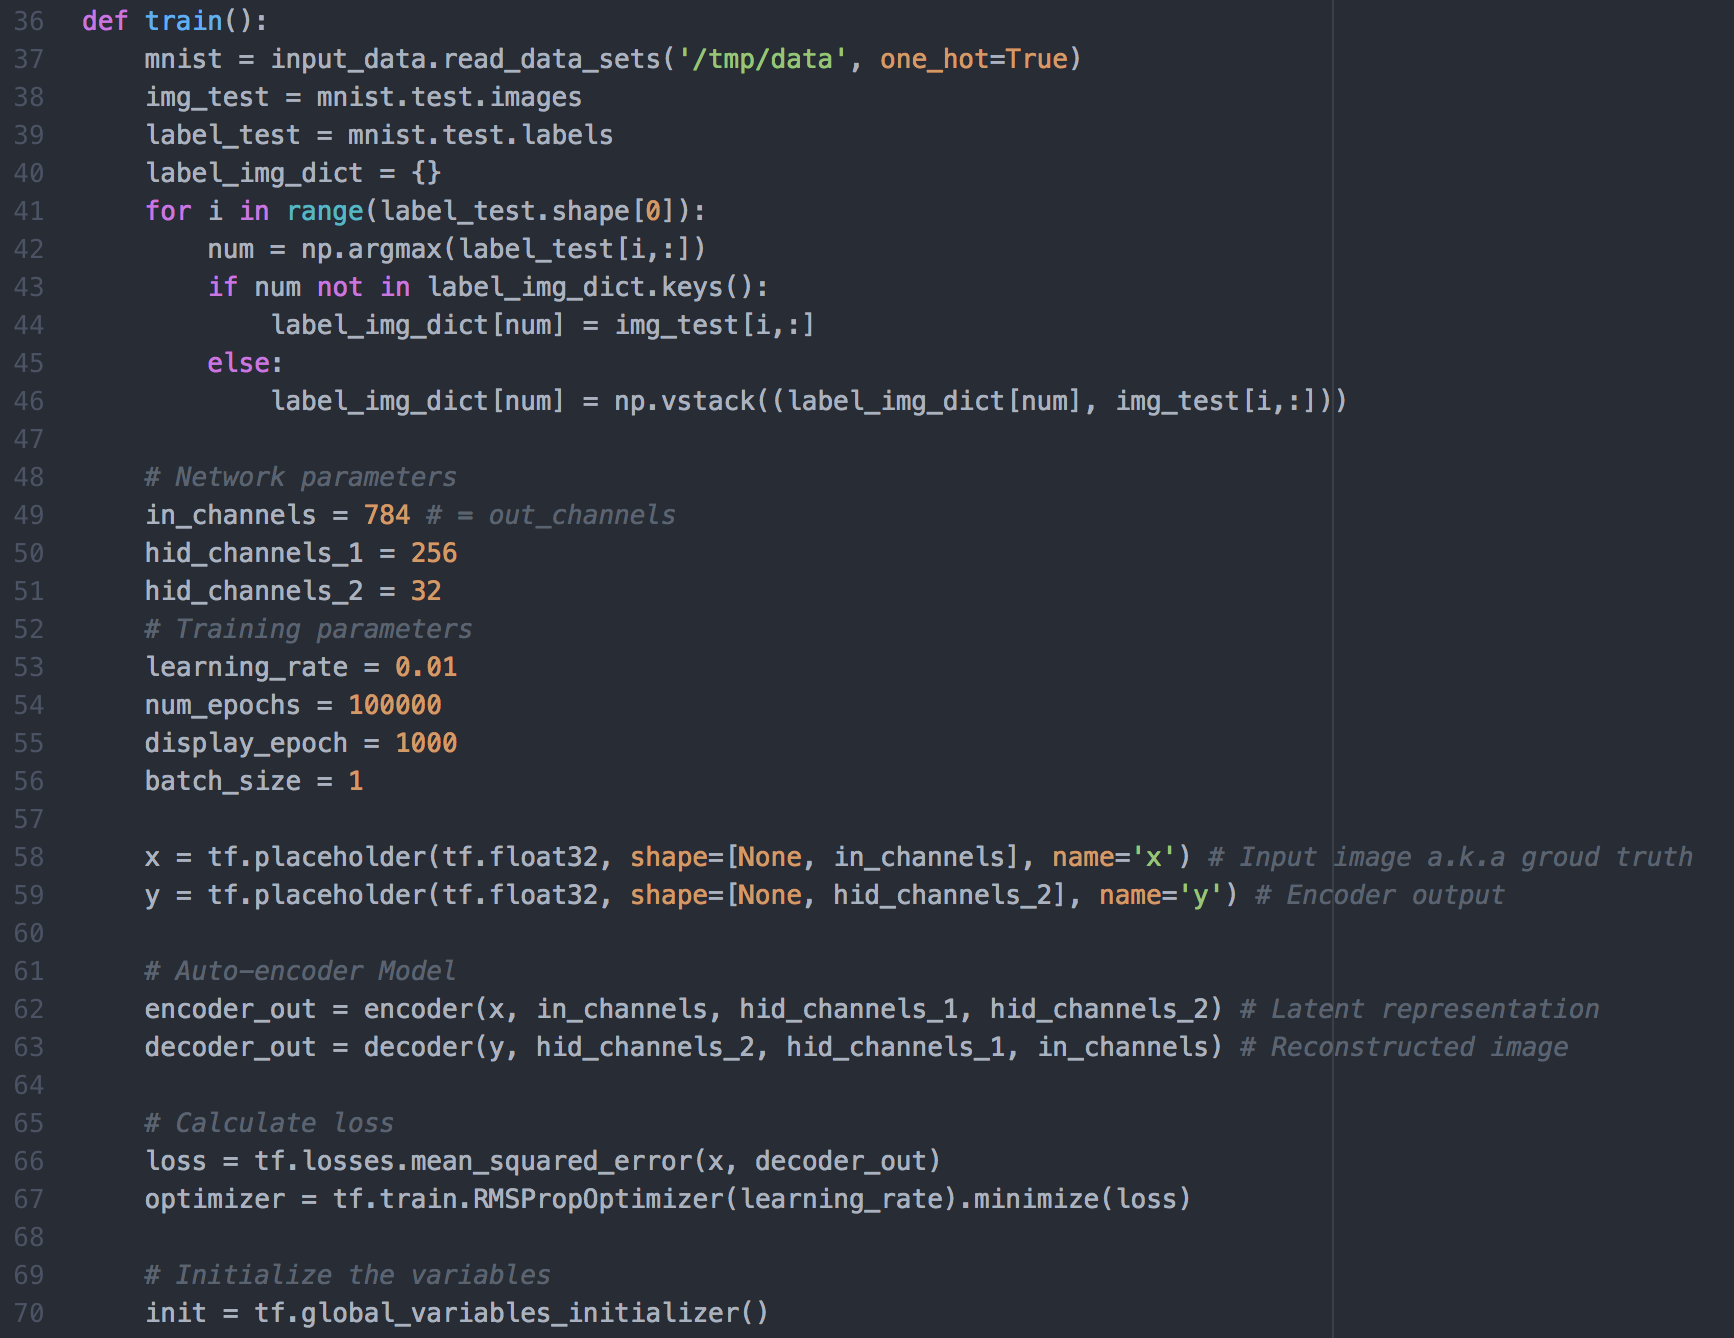
\includegraphics[width=0.9\textwidth]{2.png}
\caption{\label{fig:data}Main function.}
\end{figure}
\begin{figure}[H]
\centering
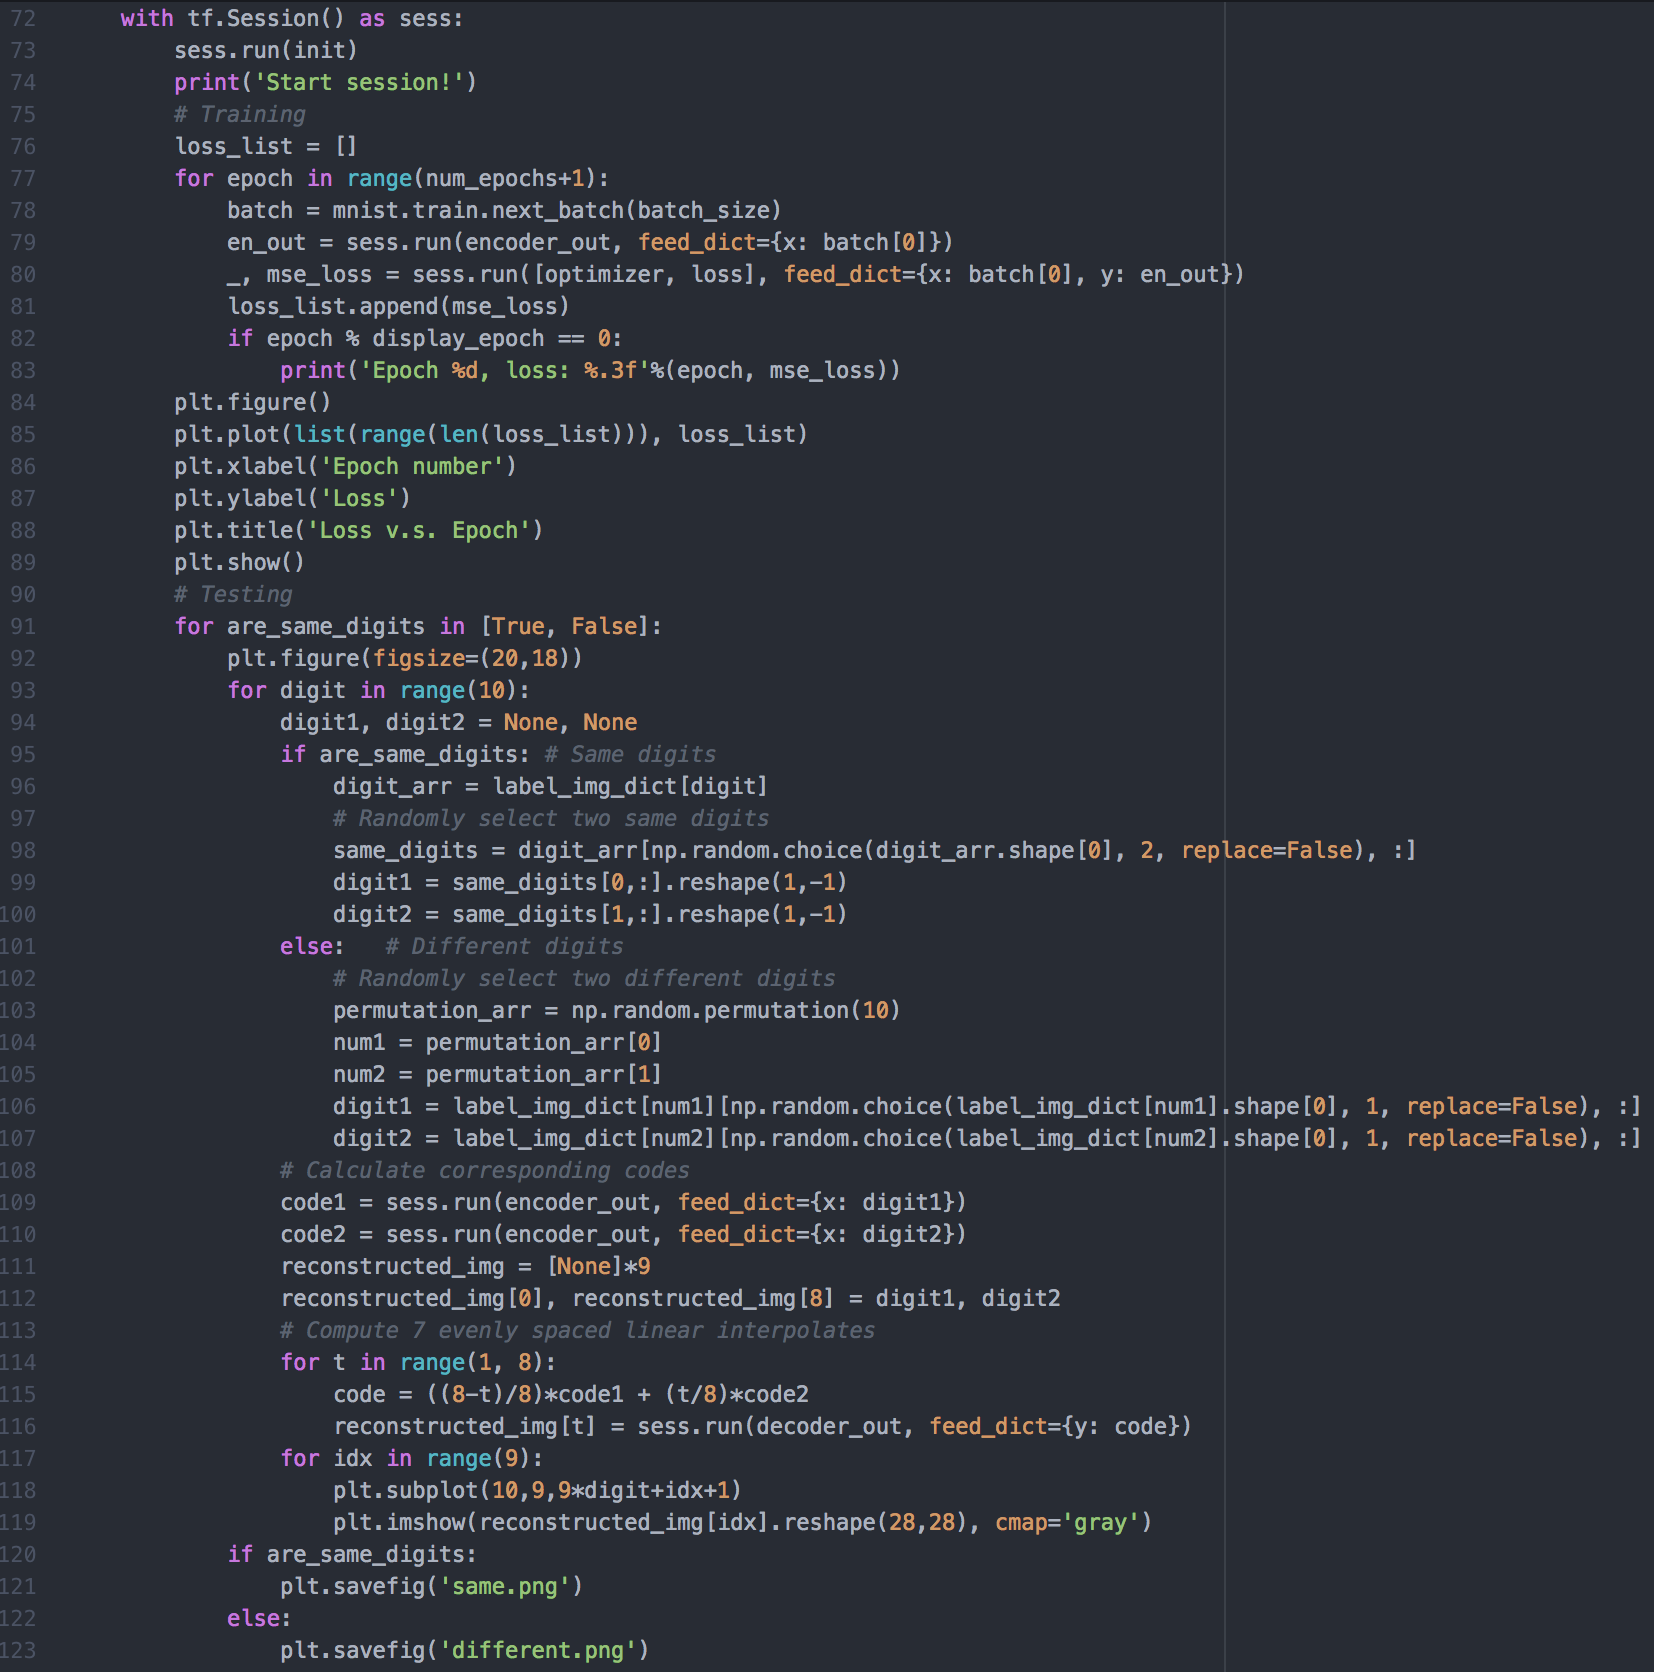
\includegraphics[width=1\textwidth]{3.png}
\caption{\label{fig:data}(Continued)Main function.}
\end{figure}

\end{document}